%!TEX root = report.tex
This section considers the results of the experiments introduced in \cref{sub:method:design}. \Cref{sub:results:interpretation} interprets the data presented in \cref{sub:results:experimental}.

\subsection{Experimental Findings}
\label{sub:results:experimental}
\Cref{fig:results:merging} presents the results of our experiments with the graph where cars had to zip merge. \Cref{fig:results:intersecting} shows the mean average speed for different routes in the graph where cars have to cross an intersection. We distinguish two different groups of routes within this graph, namely straight routes and routes that contain a bend. 

\begin{figure}
	\centering
	\begin{subfigure}{\textwidth}
		\centering
		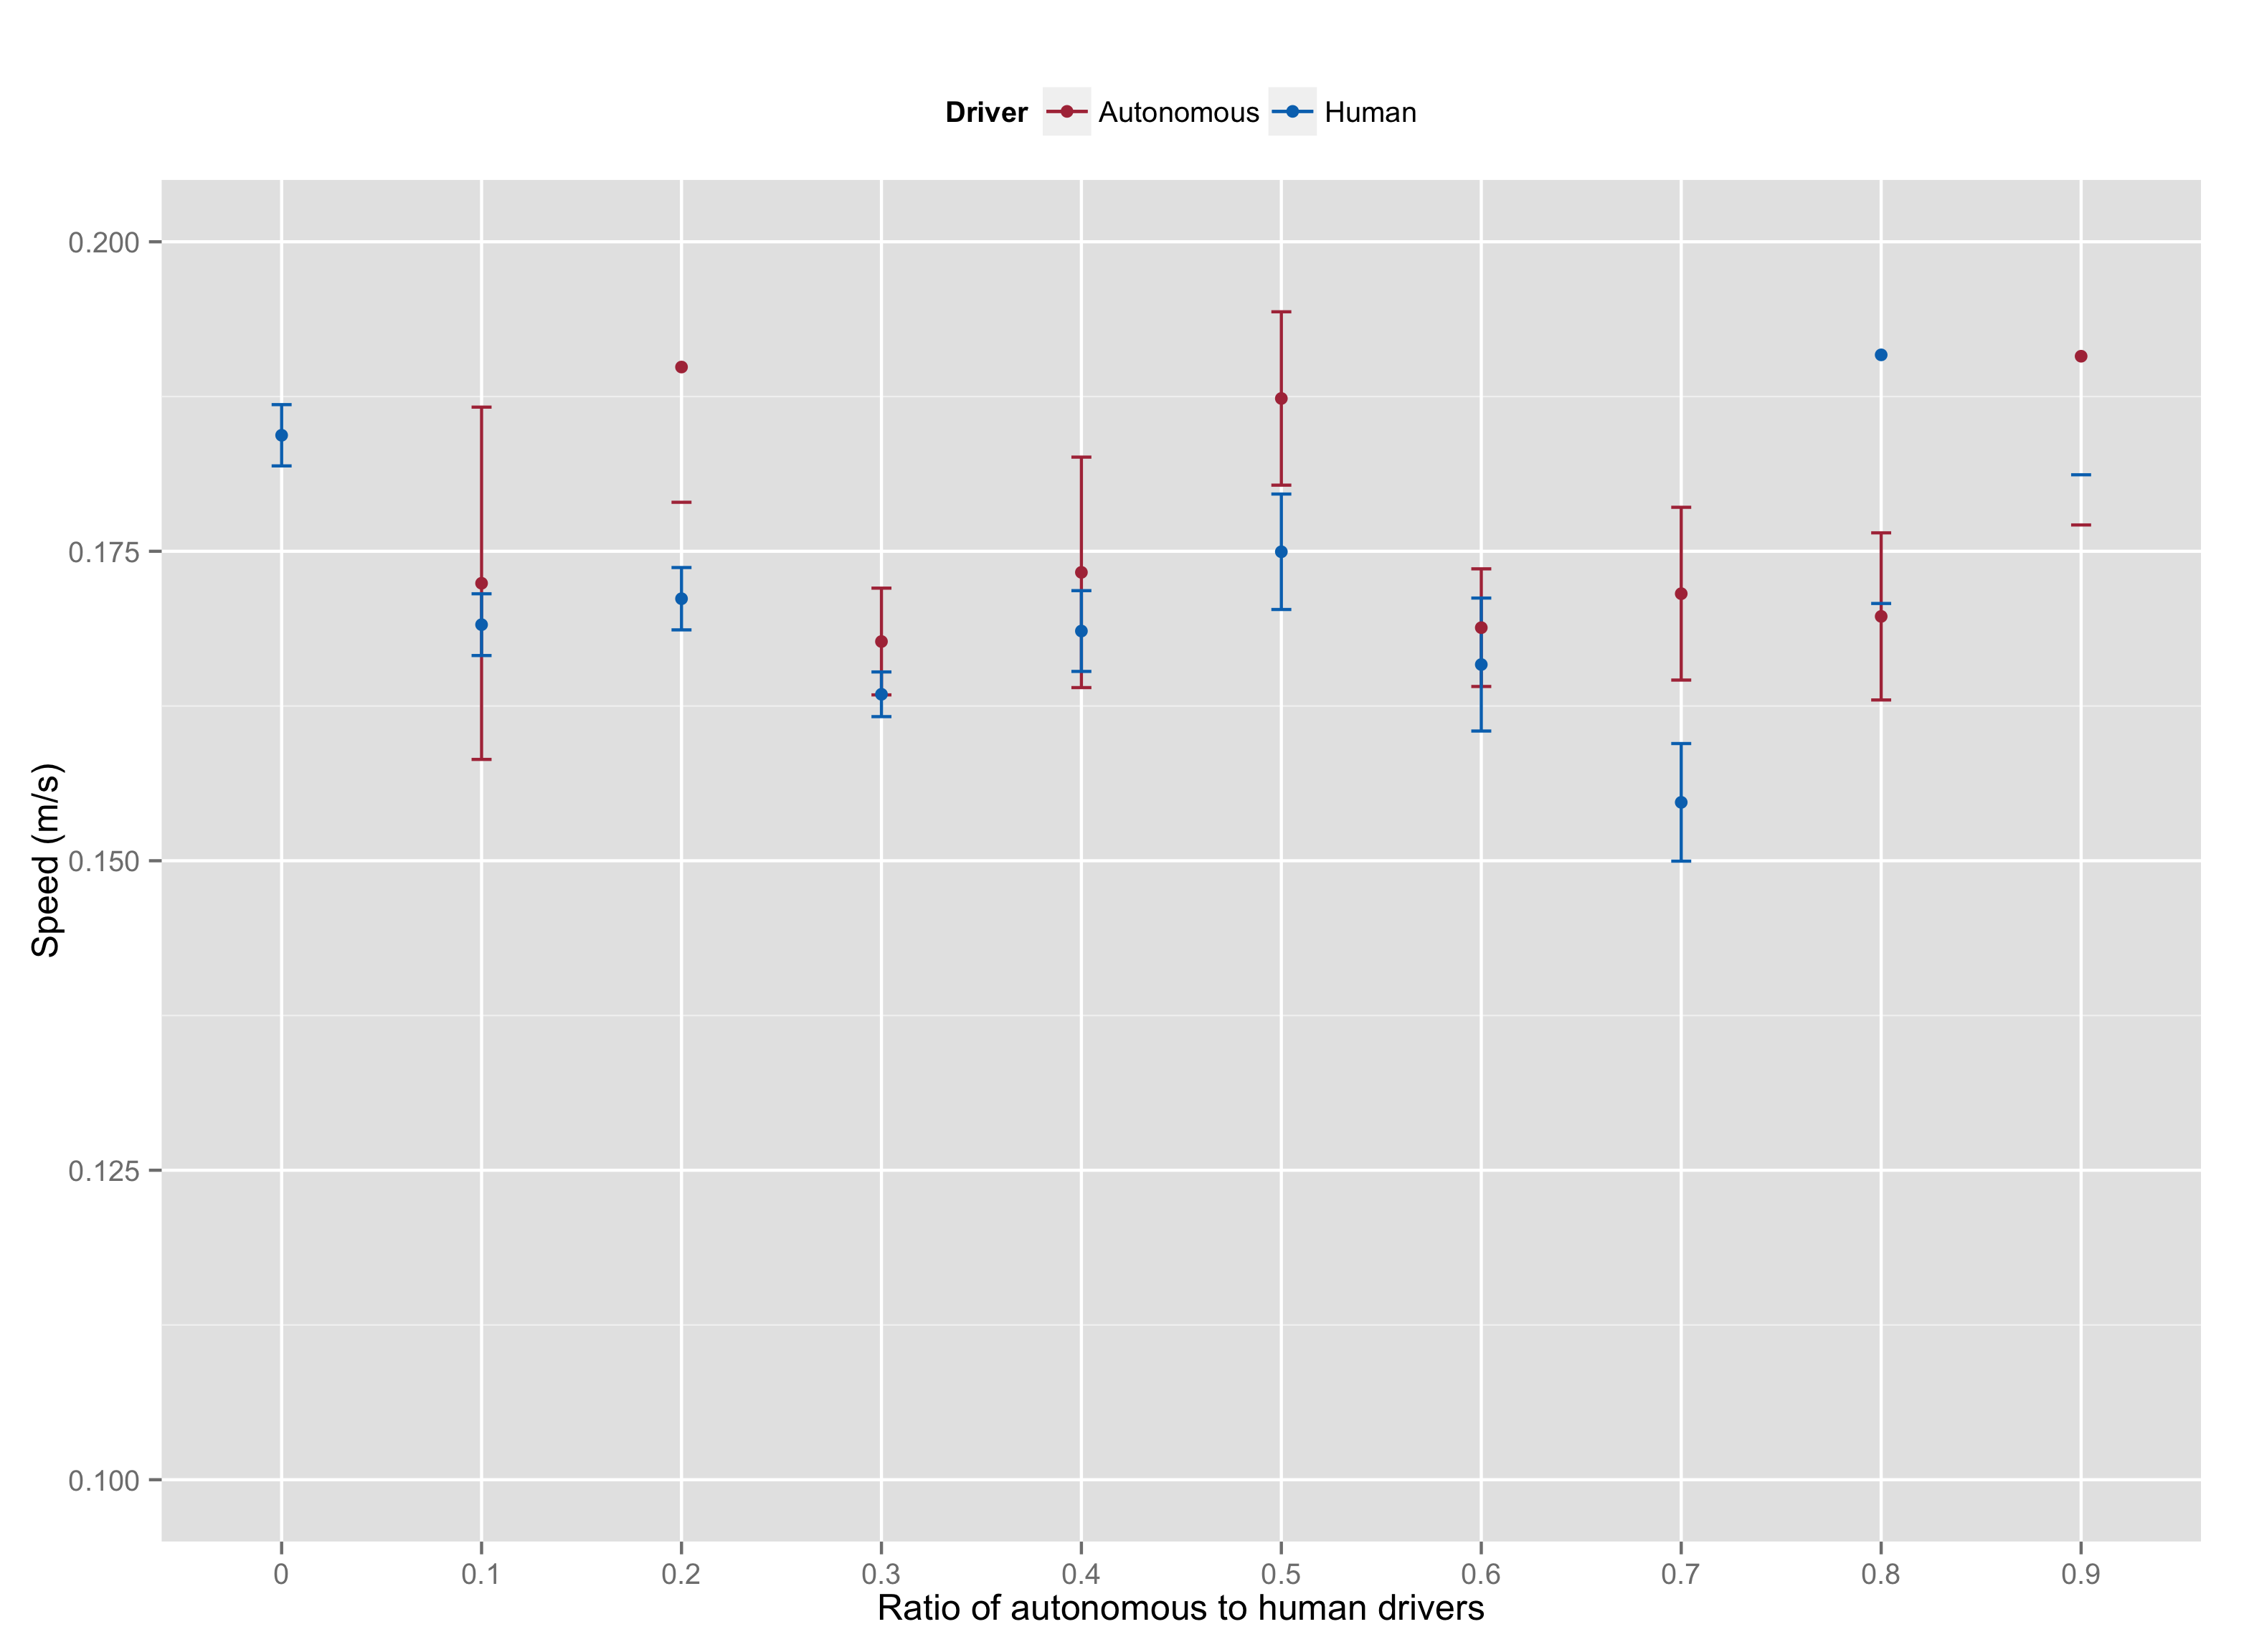
\includegraphics[width=\textwidth]{./img/results_merging_03}
		\caption{The mean average speed over the route from node $S_0$ to $S_2$.}
		\label{fig:results:merging:03}
	\end{subfigure}
	\begin{subfigure}{\textwidth}
		\centering
		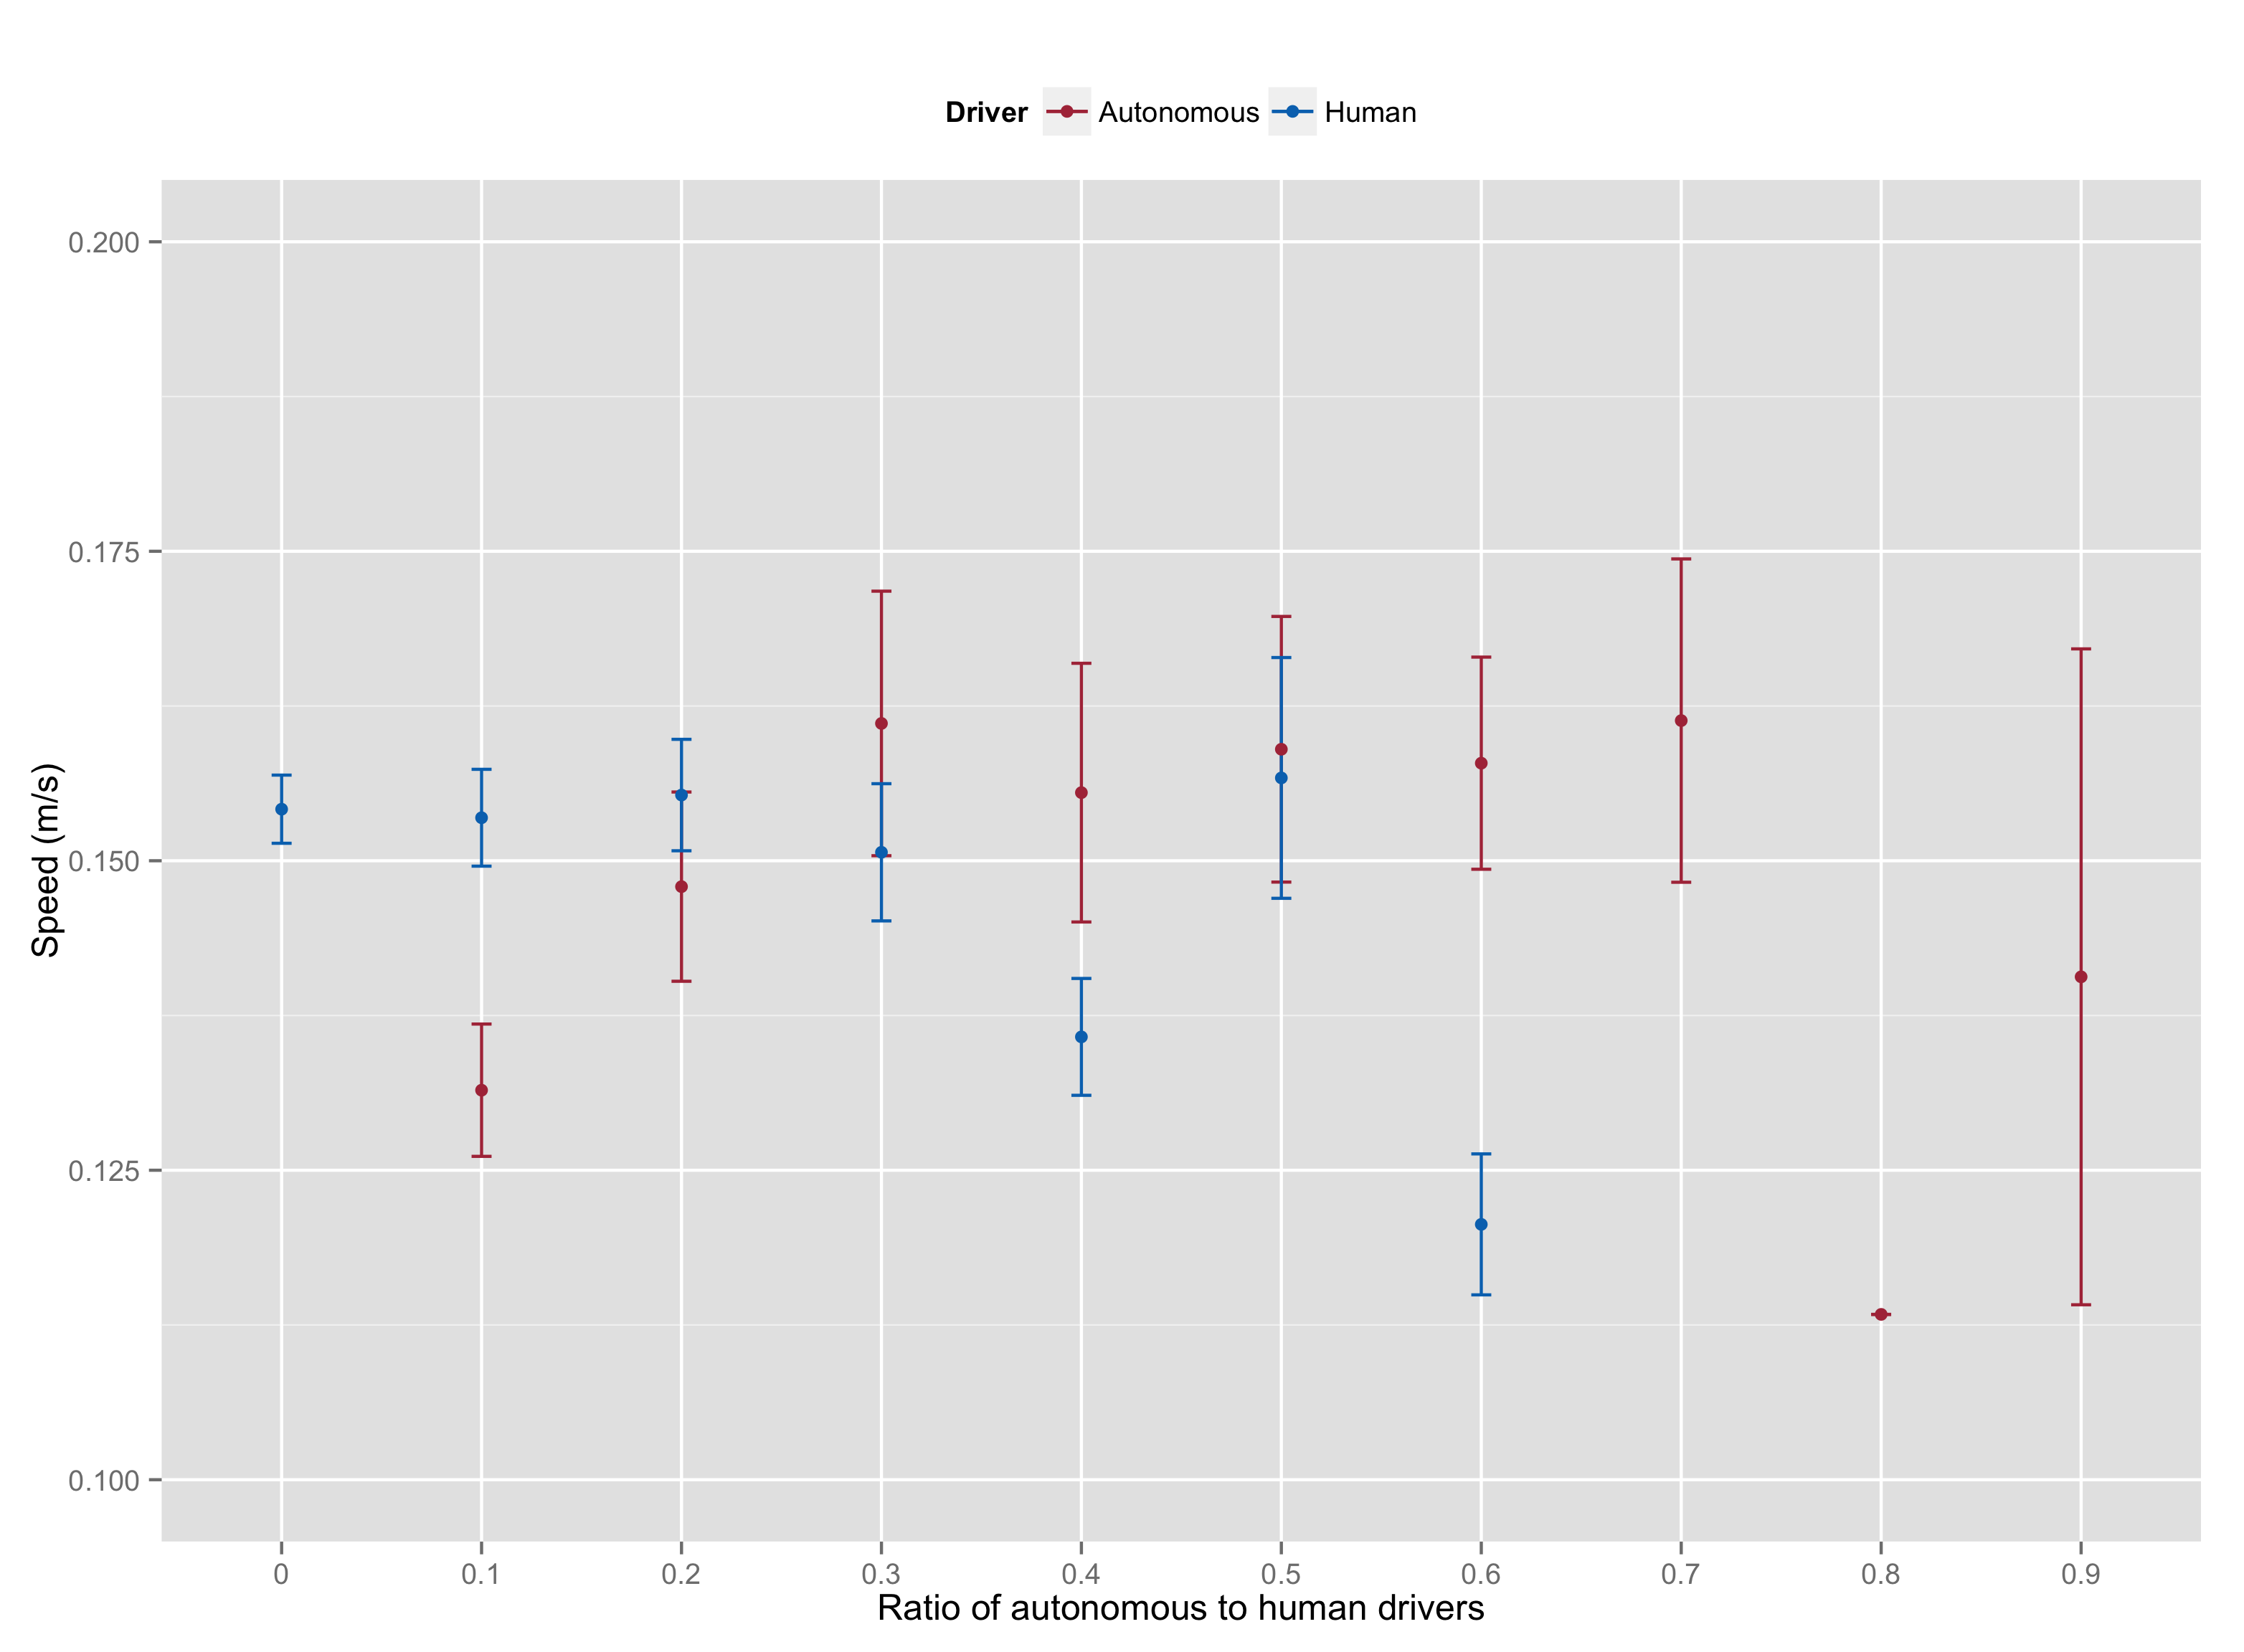
\includegraphics[width=\textwidth]{./img/results_merging_13}
		\caption{The mean average speed over the route from node $S_1$ to $S_2$.}
		\label{fig:results:merging:13}
	\end{subfigure}	
	\begin{subfigure}{\textwidth}
		\centering
		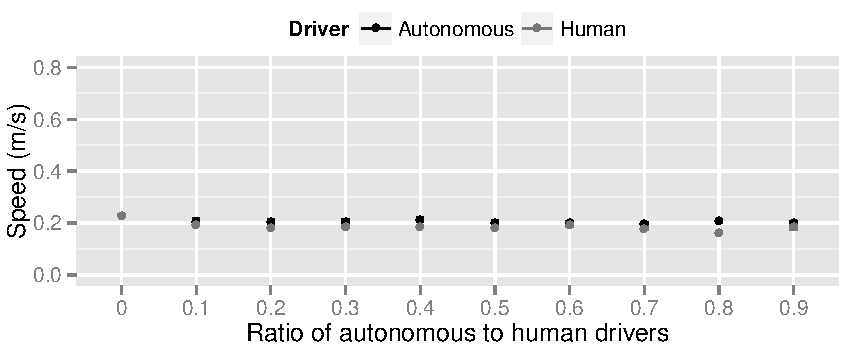
\includegraphics[width=\textwidth]{./img/results_merging}
		\caption{The mean average speed over all routes.}
		\label{fig:results:merging:all}
	\end{subfigure}		
	\caption{Mean average speed of the traffic in the `merging' graph, shown in \cref{fig:method:experiment:merging}. The bars in the plots are two standard deviations long. Each figure presents the mean average speed over different iterations as a function of the autonomous to human ratio, for a different set of routes. \ref{fig:results:merging:03} shows the mean average speed for the route from node $S_0$ to $S_2$, \ref{fig:results:merging:13} for the route from node $S_1$ to $S_2$, and \ref{fig:results:merging:all} shows the mean average speed for all routes.}
	\label{fig:results:merging}
\end{figure}

\begin{figure}
	\centering
	\begin{subfigure}{\textwidth}
		\centering
		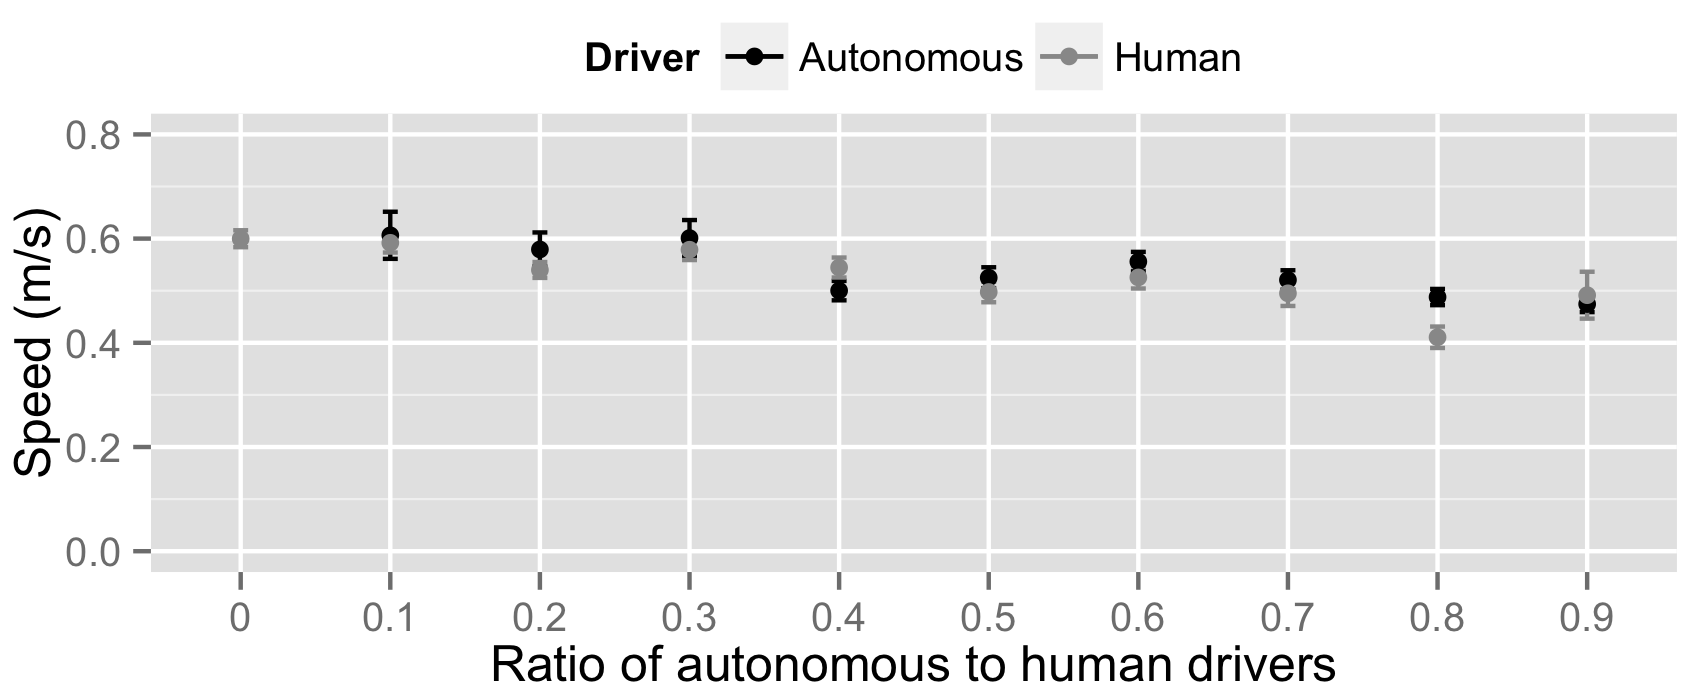
\includegraphics[width=\textwidth]{./img/results_intersecting_03_01}
		\caption{The routes from node $S_0$ to node $S_3$, $S_0$ to node $S_2$, $S_2$ to node $S_0$ and $S_3$ to node $S_0$.}
		\label{fig:results:intersecting:03}
	\end{subfigure}
	\begin{subfigure}{\textwidth}
		\centering
		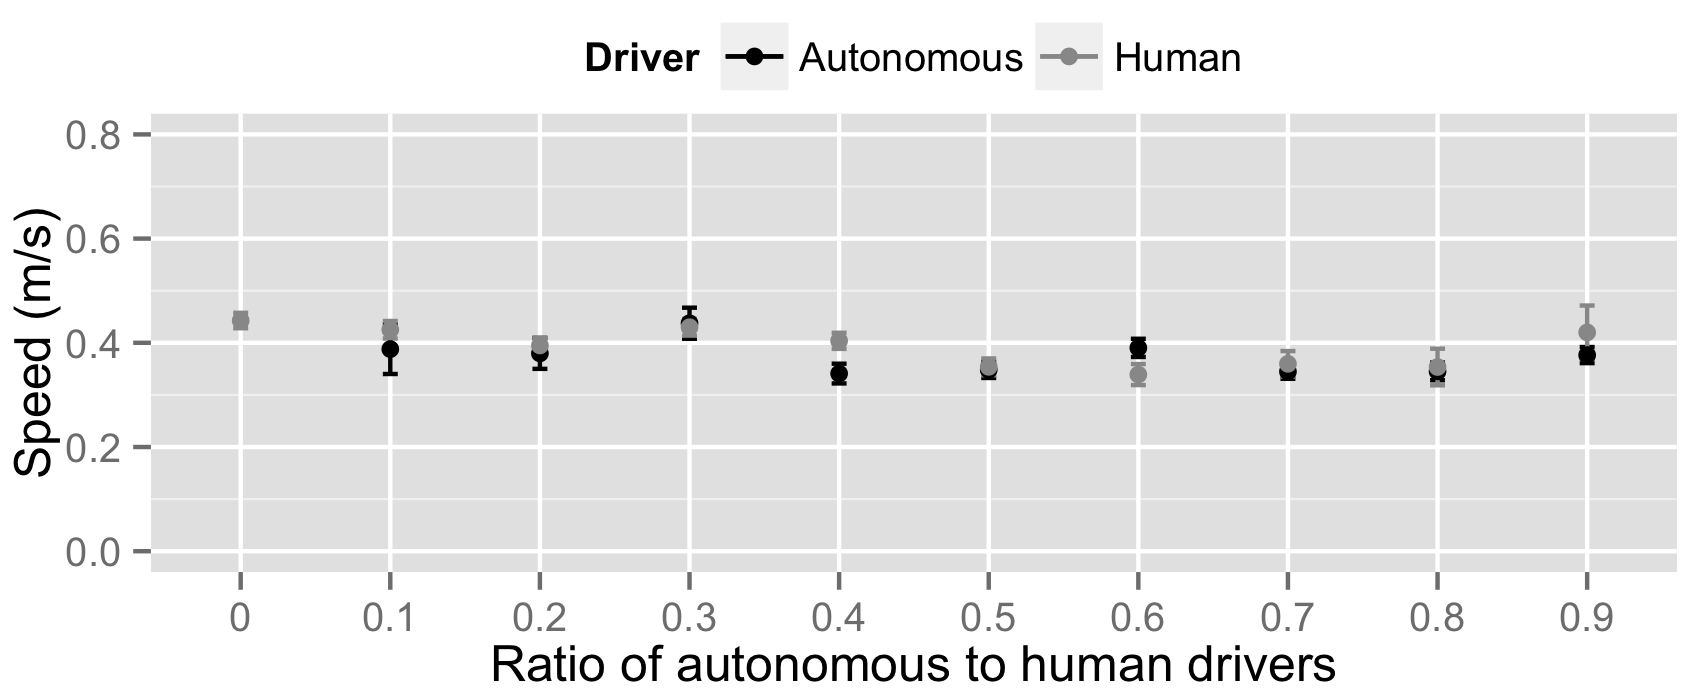
\includegraphics[width=\textwidth]{./img/results_intersecting_13}
		\caption{The route from node $S_2$ to node $S_3$ and from $S_3$ to node $S_1$.}
		\label{fig:results:intersecting:13}
	\end{subfigure}	
	\begin{subfigure}{\textwidth}
		\centering
		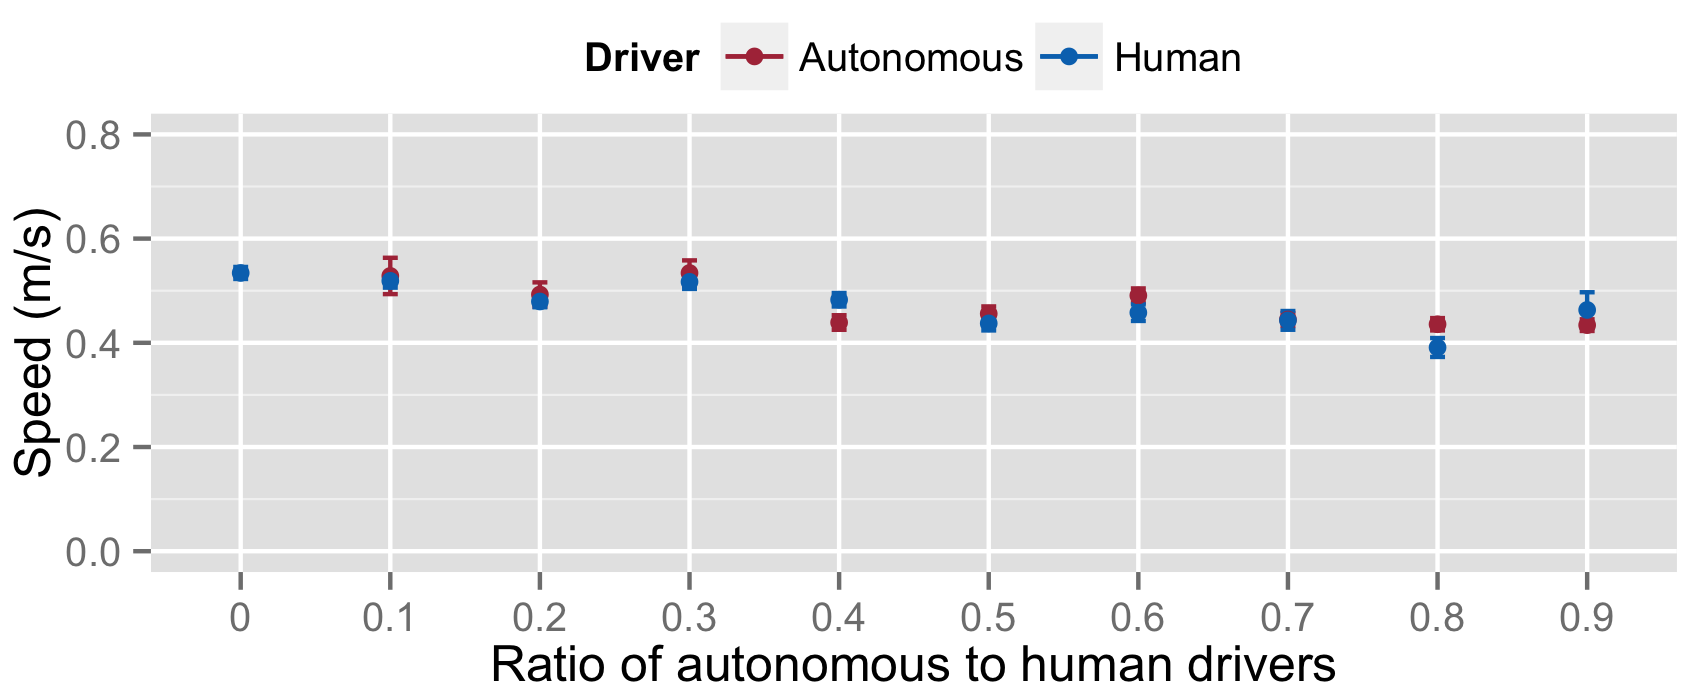
\includegraphics[width=\textwidth]{./img/results_intersecting}
		\caption{The route of all routes.}
		\label{fig:results:intersecting:all}
	\end{subfigure}		
	\caption{Results of the `intersecting' graph presented in \cref{fig:method:experiment:intersection}. The bars in the plots are two standard deviations long. Each figure presents the mean average speed over different iterations as a function of the autonomous to human ratio for a different set of routes. \ref{fig:results:intersecting:03} shows the mean average speed for the routes containing a curve, \ref{fig:results:intersecting:13} for the straight routes, and \ref{fig:results:intersecting:all} shows the mean average speed for all routes.}
	\label{fig:results:intersecting}
\end{figure}

\subsection{Interpretation of Findings}
\label{sub:results:interpretation}
%!TEX root = report.tex
The first and foremost observation from \Cref{fig:results:merging} and \Cref{fig:results:intersecting} is that the differences in average speed between human driven and autonomous vehicles are minimal. Only in \Cref{fig:results:merging:13} a noticeable difference between both types of drivers can be seen. This graph shows that the autonomous drivers are faster in passing through merging traffic than their human counterpart.

\paragraph{Differences between autonomous and human driven cars}
\Cref{fig:results:merging} shows the average speed of both types of drivers on various ratios for the Zip-merging scenario from \Cref{fig:method:experiment:merging}. Note that the total graph \Cref{fig:results:merging:all}, containing both the times from \Cref{fig:results:merging:03} and \Cref{fig:results:merging:13} shows that the autonomous drivers were barely faster than the human drivers, even though the differences on one of the routes, from vertex $S_1$ to $S_2$, is very noticeable. This is most likely an effect of the right goes first rule: cars driving along the route of $S_0$ to $S_2$ have right of way and thus more cars can drive this route.

The graphs in \Cref{fig:results:intersecting} show almost no differences between autonomous cars and human driven cars for the intersection scenario shown in \Cref{fig:method:experiment:intersection}. For both types of routes, with or without a turn, the speeds are roughly equal and whether the human drivers or autonomous cars are faster differences per ratio. No general trend can be noticed in that regard.

\paragraph{Differences between ratios}
There is no strong general trend visible in either of the two scenarios. One very weak trend they both have in common is that the higher the ratio of autonomous cars is, the lower the average speed of the traffic in total. The difference in speed between human and autonomous drivers observed in \Cref{fig:results:merging:13} might be another indicator for this: in our simulation autonomous cars seem to be slower drivers in some scenarios.

That autonomous cars seem to be slower than human drivers in the zip-merging scenario while giving right of way might be a result of their larger and circular field of view. The human driver will only see what is happening at the crossing from a distance, and not what is coming towards the crossing, due to their arc-shaped field of view. The circular field of view of autonomous cars can see more of the traffic coming towards the crossing, and will start giving right of way earlier and more often, while the human driver will be unaware and accelerate towards the crossing.
